\documentclass[12pt,a4paper]{report}

\usepackage{alltt, fancyvrb, url}
\usepackage{graphicx}
\usepackage[utf8]{inputenc}
\usepackage{float}
\usepackage{xcolor}
\usepackage{hyperref}
\usepackage{listings}

\definecolor{codegreen}{rgb}{0,0.6,0}
\definecolor{codegray}{rgb}{0.5,0.5,0.5}
\definecolor{codepurple}{rgb}{0.58,0,0.82}
\definecolor{backcolour}{rgb}{0.95,0.95,0.92}

\lstdefinestyle{mystyle}{
    backgroundcolor=\color{backcolour},   
    commentstyle=\color{codegreen},
    keywordstyle=\color{magenta},
    numberstyle=\tiny\color{codegray},
    stringstyle=\color{codepurple},
    basicstyle=\ttfamily\footnotesize,
    breakatwhitespace=false,         
    breaklines=true,                 
    captionpos=b,                    
    keepspaces=true,                 
    numbers=left,                    
    numbersep=5pt,                  
    showspaces=false,                
    showstringspaces=false,
    showtabs=false,                  
    tabsize=2
}
\lstset{style=mystyle}

\usepackage{enumitem}
\usepackage{amsmath}
\usepackage{geometry}
\geometry{margin=1in}

\usepackage{newlfont}
\usepackage{gensymb}

\usepackage[italian]{babel}
\usepackage[italian]{cleveref}

\graphicspath{ {./src/img} }

\textwidth=450pt\oddsidemargin=0pt
\begin{document}

\begin{titlepage}
\begin{center}
{{\Large{\textsc{Alma Mater Studiorum $\cdot$ Università di Bologna}}}} \rule[0.1cm]{15.8cm}{0.1mm}
\rule[0.5cm]{15.8cm}{0.6mm}
{\small{\bf CORSO DI LAUREA IN INGEGNERIA E SCIENZE INFORMATICHE \\ A.A. 2024/25 }}
\end{center}
\vspace{15mm}
\begin{center}
{\LARGE{\bf Analisi del traffico ICMP e TCP}}\\
\vspace{2mm}
{\LARGE{\bf con Scapy e Wireshark}}
\end{center}
\begin{center}
{\LARGE Relazione per il corso di Programmazione di Reti}
\end{center}

\vspace{8mm}
\begin{center}

\includegraphics[width=0.7\textwidth]{Copertina}
\end{center}
\vspace{15mm}

{\large{\bf \noindent
Presentato da:\\}
Bartocetti Enrico, 0001115097}
\end{titlepage}

\tableofcontents

\chapter{Introduzione}

\subsubsection{Obiettivo}
Creare e inviare pacchetti ICMP e TCP con Scapy, catturarli con Wireshark e analizzare i risultati.

\subsubsection{Requisiti minimi}
\begin{itemize}
	\item Inviare pacchetti ICMP Echo (ping) e TCP SYN verso un host
	\item Catturare i pacchetti in Wireshark e salvarli in .pcap
	\item Analizzare: IP di origine/destinazione, porte, checksum, TTL
\end{itemize}

\subsubsection{Estensioni opzionali}
\begin{itemize}
	\item Inviare un pacchetto TCP con flag personalizzati
	\item Visualizzare e spiegare le differenze tra ICMP e TCP
	\item Generare un semplice report HTML o PDF con gli screen e analisi
\end{itemize}

\subsubsection{Output atteso}

\begin{itemize}
	\item Script Python con Scapy
	\item File .pcap della cattura
	\item Relazione con screenshot e commenti tecnici
\end{itemize}

\chapter{Pacchetti ICMP Echo}

\section{Generazione dei pacchetti con Scapy}

Si vuole inviare un pacchetto \texttt{ICMP Echo Request} (ping) a un host. Per l'invio ho utilizzato il metodo \texttt{.sr} della libreria scapy, specificando il tipo \texttt{ICMP}. Riporto nel Listing \ref{code:icmp} la funzione che ho scritto per poter generare il pacchetto del ping, che richiede come parametro l'indirizzo IP oppure l'hostname del destinatario. La funzione stampa anche il risultato dell'operazione.

\begin{lstlisting}[language=Python, caption={Funzione python per la generazione di un pacchetto \texttt{ICMP Echo Request}}, label={code:icmp}]
import scapy.all as scapy

def send_ping(destination):
    print("----- INVIO PING A", destination, " -----")
    res = scapy.sr(scapy.IP(dst=destination)/scapy.ICMP(), timeout=4) 
    print("--- RISULTATI: ---")
    for r in res:
        r.show()
    print()
\end{lstlisting}

\section{Analisi del traffico con Wireshark}
Ho mandato il ping a \texttt{google.com}, che è stato risolto nell'indirizzo IP \texttt{216.58.204.238}.\\
Per la cattura del traffico di rete ho utilizzato wireshark con il filtro \texttt{host 216.58.204.238} per catturare solo i pacchetti da / per l'host indicato. Nel file \texttt{wireshark/icmp{\textunderscore}echo.pcap} è presente il risultato della cattura. \\
Riporto in seguito il dettaglio della richiesta e della risposta.

\subsection{ICMP Echo Request}
\begin{figure}[H]
	\centering
	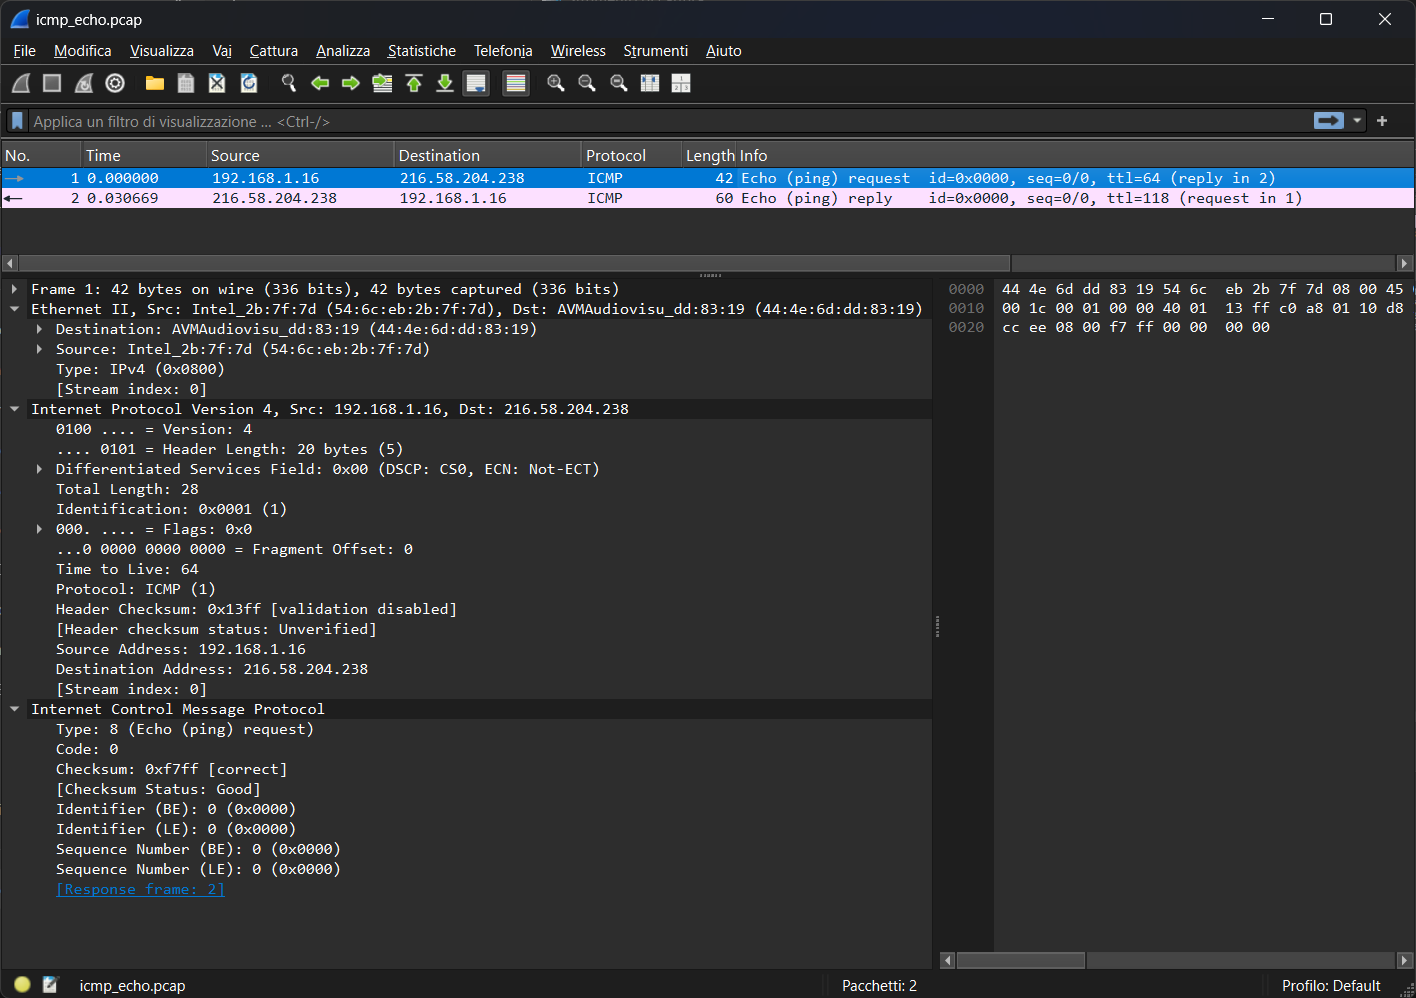
\includegraphics[width=1\textwidth]{icmp_echo_request}
 	\caption{Dettaglio Wireshark dell'Echo Request}
\end{figure}
Il pacchetto parte dal mio PC connesso alla rete di casa, infatti nella PCI del livello IP troviamo il campo \texttt{Source Address: 192.168.1.16}, ovvero l'IP privato del mio PC nella mia rete. Nel campo \texttt{Destination Address: 216.58.204.238} troviamo l'IP del destinatario della richiesta, ovvero l'host verso cui ho inviato il pacchetto ping. Il campo Time To Live è settato al livello massimo (64) visto che il pacchetto è stato catturato non appena generato.\\
Nella parte dati del pacchetto IP viene trasportato il pacchetto ICMP: possiamo confermarlo leggendo il campo \texttt{Protocol: ICMP} nell'header del pacchetto IP. All'interno della parte riservata al protocollo ICMP viene specificato che il pacchetto è di tipo \texttt{Echo Request}.\\
Notiamo che non sono presenti riferimenti a nessuna porta: questo perché IP e ICMP sono protocolli dell'Internet Layer della suite TCP/IP , quindi non c'è la necessità di comunicare tramite una porta con un livello superiore (ovvero con un protocollo di trasporto).\\
Risulta infine evidente che sia il pacchetto IP sia quello ICMP sono dotati di un proprio checksum, che nel caso dell'IP non viene verificato mentre nell'ICMP è corretto. 

\subsection{ICMP Echo Reply}
\begin{figure}[H]
	\centering
	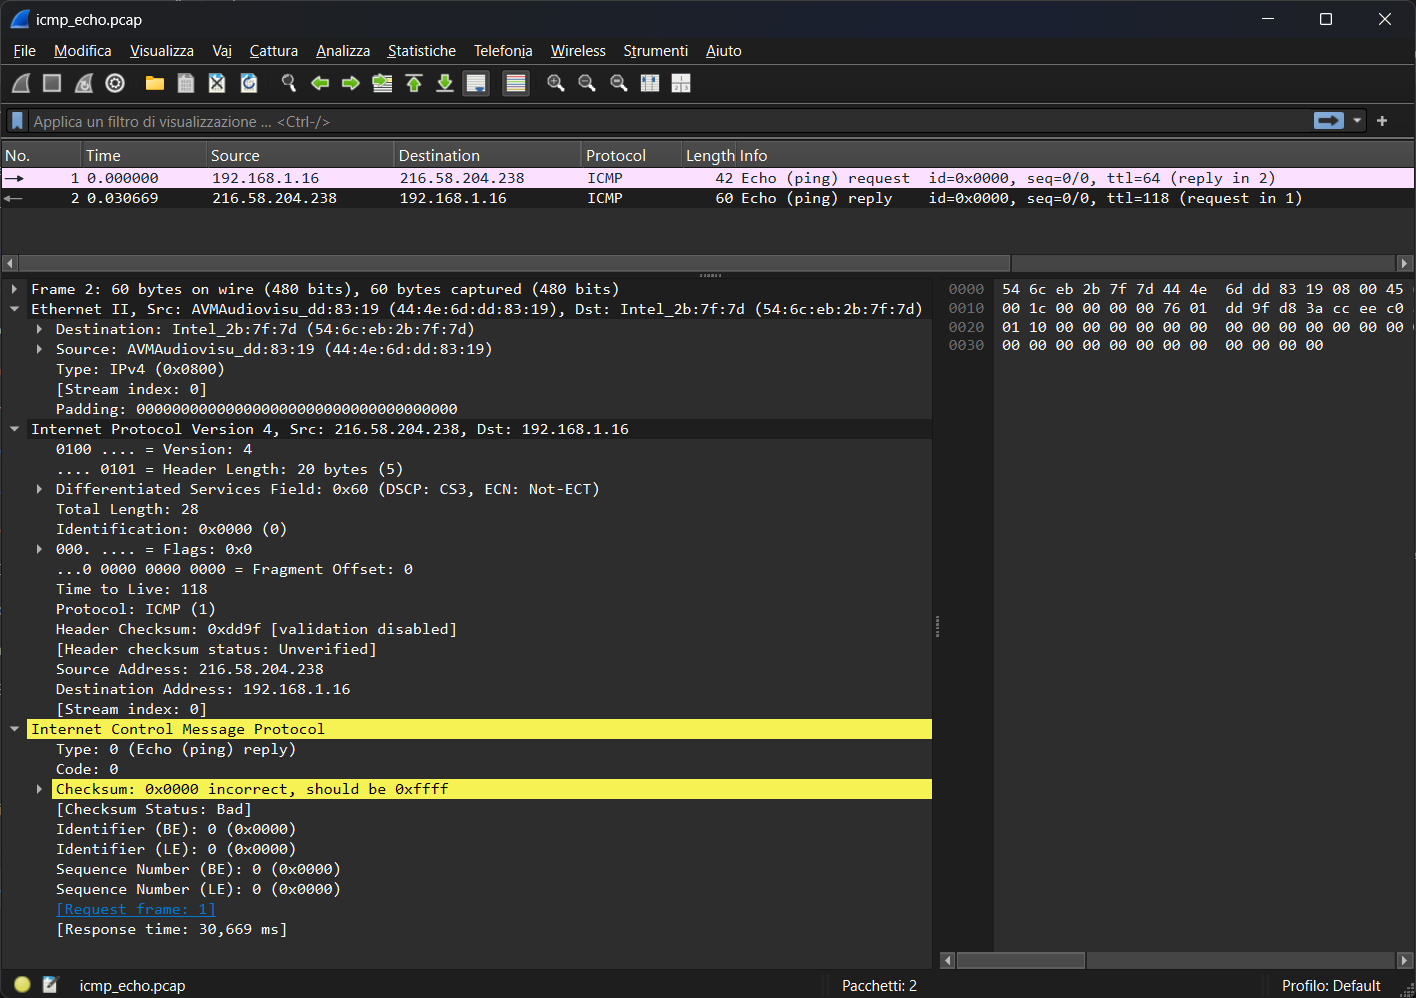
\includegraphics[width=1\textwidth]{icmp_echo_reply}
 	\caption{Dettaglio Wireshark dell'Echo Reply}
\end{figure}
Questa cattura presenta varie differenze rispetto a quella precedente. 
Quella più ovvia è l'inversione degli indirizzi IP nei campi \texttt{Destination Address: 192.168.1.16} e  \texttt{Source Address: 216.58.204.238}, visto che si tratta del pacchetto di risposta (quindi generato dal destinatario del ping).\\
Poiché si tratta della risposta al ping iniziale, IP ci dice che il protocollo utilizzato è sempre \texttt{Protocol: ICMP}, mentre nella parte riservata al protocollo ICMP viene specificato che si tratta di una \texttt{Echo Reply}.\\
In questo caso il campo {TTL} è settato a 118: possiamo presupporre che alla generazione del pacchetto sia stato 128 (la potenza del 2 più vicina a 118), ma è stato decrementato di un'unita per ogni router che il pacchetto ha attraversato.
Utilizzando il comando \texttt{tracert 216.58.204.238} ho poi verificato che per raggiungere il destinatario dal mio host sono necessari 10 salti. \\
Come prima il checksum dell'header IP è presente ma non verificato. Nel caso di ICMP invece, si ha che il checksum calcolato è diverso da quello riportato nel pacchetto. Ho provato a ripetere varie volte il ping, ottenendo sempre lo stesso risultato: potrebbe quindi essere che l'host destinatario sceglie di non calcolare il checksum lasciandolo a 0. Il contenuto informativo del pacchetto sembra comunque essere corretto nei campi che sono di nostri interesse.

\chapter{Segmenti TCP SYN}

\section{Generazione dei segmenti}
\section{Analisi del traffico con Wireshark}

\chapter{Segmenti TCP con flag personalizzati}

\section{Generazione dei segmenti}
\section{Analisi del traffico con Wireshark}

\end{document}